Research on various aspects of hovercraft design, mechanics and physics first principles, as well as input from the TA and the design decisions of our peers, led us to our own hovercraft design. This document first describes the information we uncovered about the mechanics of a hovercraft, then proceeds by describing our design and summarizing our final product.

\subsection{Hovercraft Mechanics}
The hovercraft is able to move freely due to the minimum amount of friction between the vehicle and the ground. The chamber of air between the craft and ground, called the plenum chamber, is formed by the body of the hovercraft and a skirt. The air flowing into the plenum chamber forms a ring which keeps the external lower pressure out, ensuring the persistence of the internal air cushion. The amount of air entering the plenum chamber must be at least be equal to the amount of air that escapes underneath the skirt in order to keep the craft afloat. Further, it is incorrect to assume that air will escape evenly around the skirt’s perimeter. As more air is blown into the plenum chamber, the pressure of the air on the inside becomes higher than that on the outside, creating an upward force that lifts the hovercraft. When this upward pressure exactly matches the downward force of gravity, the desired floating effect is achieved.

\subsubsection{Steering}
Different approaches have been taken to steer the craft. Larger hovercrafts typically employ a large propeller at the rear to drive the vehicle forward. Rudders are used for steering. Another option, usually seen in smaller hovercrafts, is to tilt the base, affecting the plenum chamber underneath. This results in a change in direction because a drag is created on one side, creating a pivot point.


  \begin{center}
    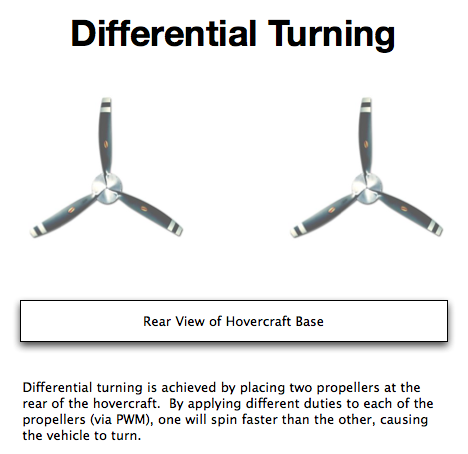
\includegraphics[width=85mm]{imageSources/differentialTurning.png}
  \end{center}
  \captionof{figure}{Differential Turning} 
  \label{differentialTurning}


Instead of using 2 fans on the craft (one for filling the plenum chamber and one for forward thrust), a single propeller may be used for both functions. A fraction of the air intake is directed into the inner chamber to lift the craft, while the remaining air flow is forced behind the craft, creating thrust.


  \begin{center}
    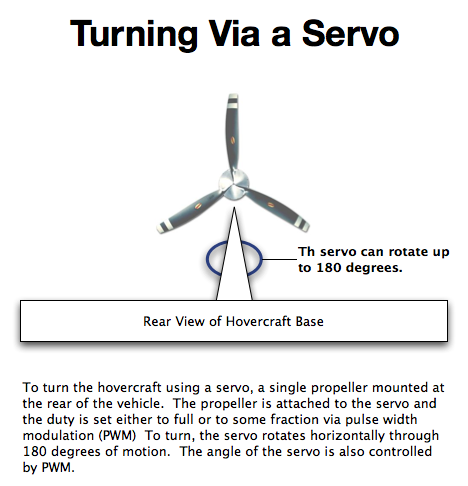
\includegraphics[width=85mm]{imageSources/servoTurning.png}
  \end{center}
  \captionof{figure}{Servo Turning} 
  \label{servoTurning}


Steering may further be affected by either differential turning or though the use of a servo motor. The former approach commonly employs two thrust sources on either side of the vehicle. By altering the thrust of either motor (for example with pulse width modulation), one motor will be more powerful than the other, causing the craft to turn. The latter approach sees a propeller mounted to a servo motor. As the servo rotates through its 180 degree range, the thrust of the propeller is directed in a specific direction, also causing the craft to turn.

\subsubsection{Skirt}
An advancement in the development of the skirt is known as the Double-Walled Flexible Skirt, or more commonly the “Big Skirt”. The design came about in the 1960’s by McReary. The idea was to inflate the outer skirt to allow the craft to move more freely over rough terrain and choppy water.

In general, the purpose of the skirt is to increase the overall surface area of the vehicle. By spreading the weight of the craft over a lager area, the pressure required to counteract this downward pressure is reduced. A common analogy is that of stepping on a single nail as opposed to lying on a bed of nails. Applying one’s entire weight on the small surface area of a single nail will surely result in a painful experience. However, by spreading one’s weight over the combined surface area of many nails, the pressure on any single point is reduced to the point where any particular nail cannot cause harm.

\subsection{Ground Effect}
Ground effect refers to the collection of aerodynamic effects felt by aircraft when flying in close proximity to the ground. If the hovercraft has too much lift, it is likely that it may well feel the effects of such a phenomenon.


  \begin{center}
    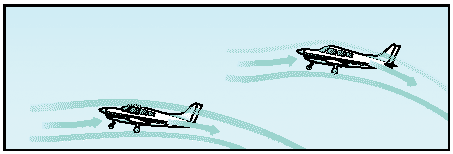
\includegraphics[width=85mm]{imageSources/groundEffect.png}
  \end{center}
  \captionof{figure}{Ground Effect Airflow} 
  \label{groundEffect}

One of the most prominent is the Wing-In-Ground effect, whereby the aircraft experiences reduced amounts of drag when flying at an altitude less than the length of its wingspan. Though the physics are somewhat complicated and beyond the scope of this report, the result is an increase in speed and lift when flying in ground effect. Ground effect is more significant for lighter aircraft than for heavier aircraft. Ground effect also has implications for rotary aircraft like helicopters. They require less energy to remain air bourn while in ground effect.

\subsection{Vortex Ring Effect}
Another interesting property of propellers, such as those used in Helicopters, is Vortex Ring effect. As helicopter blades spin, they direct air downwards, creating lift. Sometimes this air may recycle, looping around and reentering the blades. This can have a drastic effect on lift.

\begin{figure}[h]
  \begin{center}
    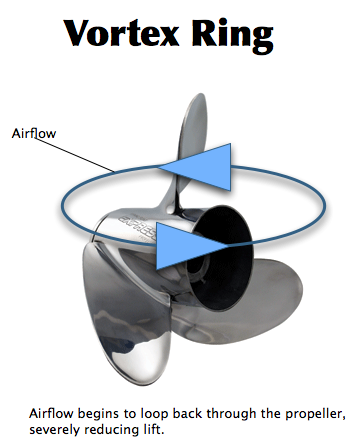
\includegraphics[width=85mm]{imageSources/vortexRing.png}
  \end{center}
  \caption{Vortex Ring Effect} 
  \label{vortexRing}
\end{figure}

\subsection{Design Schematics}

The following figures show the top, side, front and rear views for the vehicle:

\begin{figure}[h]
  \begin{center}
    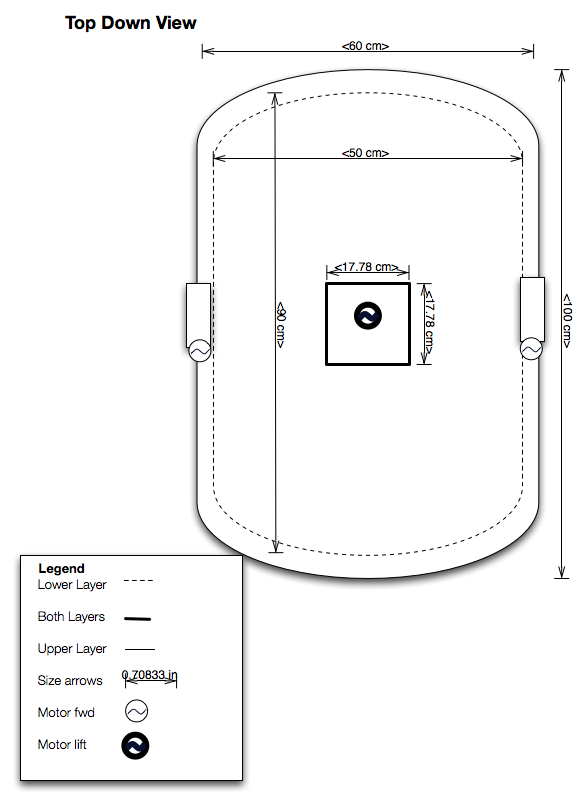
\includegraphics[width=85mm]{imageSources/topDownView.png}
  \end{center}
  \caption{Hovercraft: Top Down View} 
  \label{topDownView}
\end{figure}

The first design consisted of a rounded front, straight sides and a straight back. However, since the front and back were not symmetric, we concluded that the rear of the craft should be rounded to match the front. This symmetric design better distributes the underlying air cushion to all parts of the vehicle.

\begin{figure}[h]
  \begin{center}
    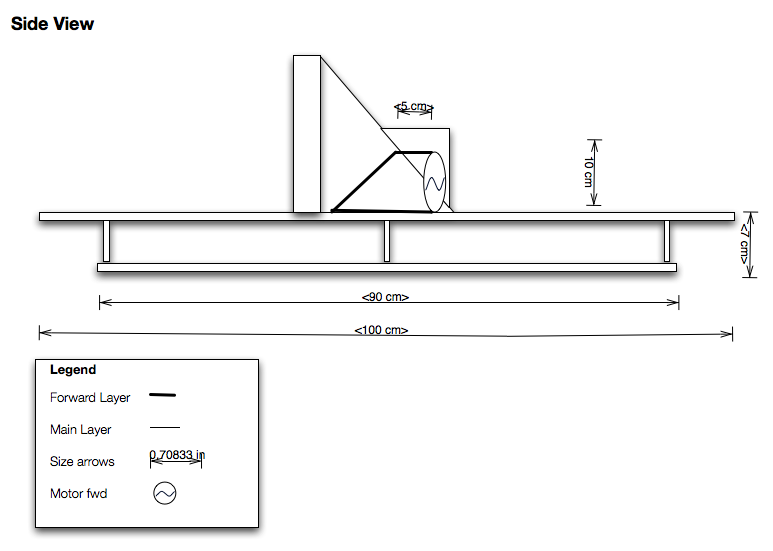
\includegraphics[width=85mm]{imageSources/sideView.png}
  \end{center}
  \caption{Hovercraft: Side View} 
  \label{sideView}
\end{figure}

The plenum chamber receives air from a single propeller mounted in the middle of the chasis. The middle propeller is housed by a triangular container. Initially the container was completely open on the side where the propeller draws air from. We realized that too much air was escaping from this hole and a cover with a circular cut-out was fitted over the opening. The cut-out better fit the diameter of the fan, resulting in minimal air escaping from the opening.

\begin{figure}[h]
  \begin{center}
    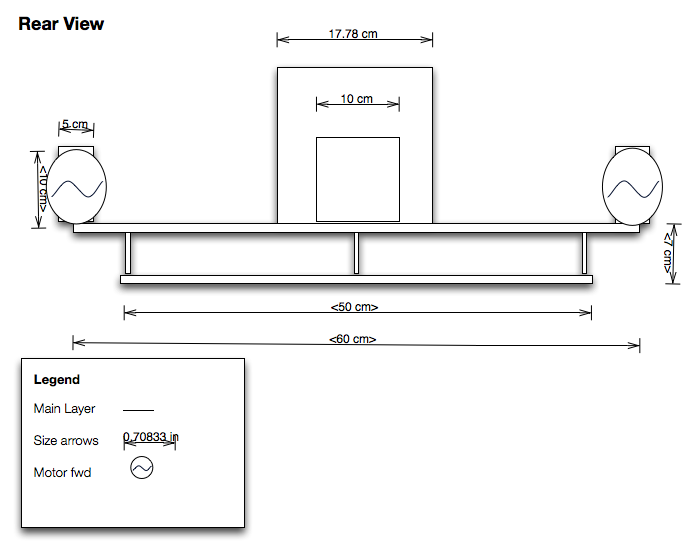
\includegraphics[width=85mm]{imageSources/rearView.png}
  \end{center}
  \caption{Hovercraft: Rear View} 
  \label{rearView}
\end{figure}

The electronic components are mounted at the rear of the hovercraft. This facilitates making connections from the breadboard to the nearby DC Motors, servo motor, and sonars. The combined mass of all the components added a significant force to the rear of the chasis. To counter this, we placed counter weights on the front of the body.

\begin{figure}[h]
  \begin{center}
    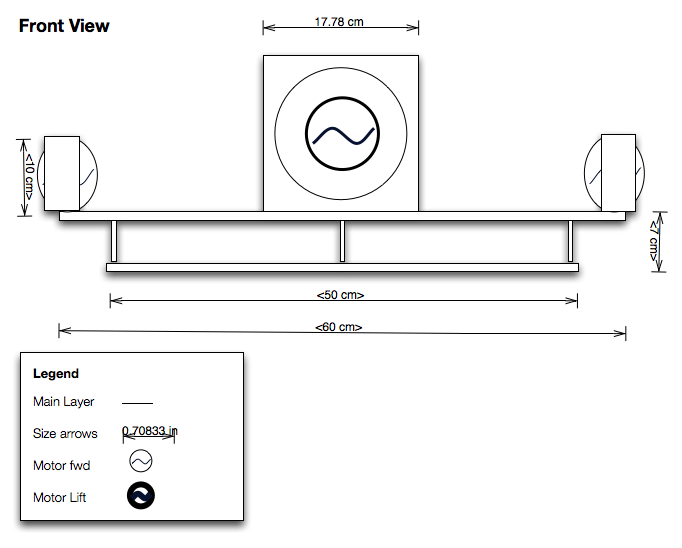
\includegraphics[width=85mm]{imageSources/frontView.png}
  \end{center}
  \caption{Hovercraft: Front View} 
  \label{frontView}
\end{figure}

\subsection{Design Constraints}
The following constraints were issues that needed to be met by the resulting hovercraft design.

\subsubsection{Payload Weight}
In order for the hovercraft to stay afloat, the internal air pressure must counter external forces placed on the surface of the vehicle by both gravity and the mass of the components. The following table describes the components and their masses:

\begin{table}
\caption{Weight of Hovercraft Components}
\begin{center}
\begin{tabular}{ c c c}
  Component & Quantity & Weight (grams) \\
  \hline
	Battery  &	2 & 	50 \\
	Breadboard &	1 &	45 \\
	Microcontroller &	1 &	15 \\
	Radio &	1 &	9 \\
	Sonar &	3 &	5 \\
	DC Motor (large) &	1 &	83 \\
	Servo Motor &	1 &	4 \\
	H-bridge &	1 &	6 \\
	DC Motor (small) &	2 &	25 \\
	Total &	-- &	329 \\
\end{tabular}
\end{center}
\label{restingTable}
\end{table}

\subsection{Rigidity}
The hovercraft body is made from two thin sheets of styrofoam separated by 12 styrofoam spacers 1'' thick. This has proven to be a very strong design, easily capable of supporting the payload of the electronics. In fact, we distributed additional weight evenly across the body and found that the hovercraft could support at least 1 kg.

\begin{figure}[h]
  \begin{center}
    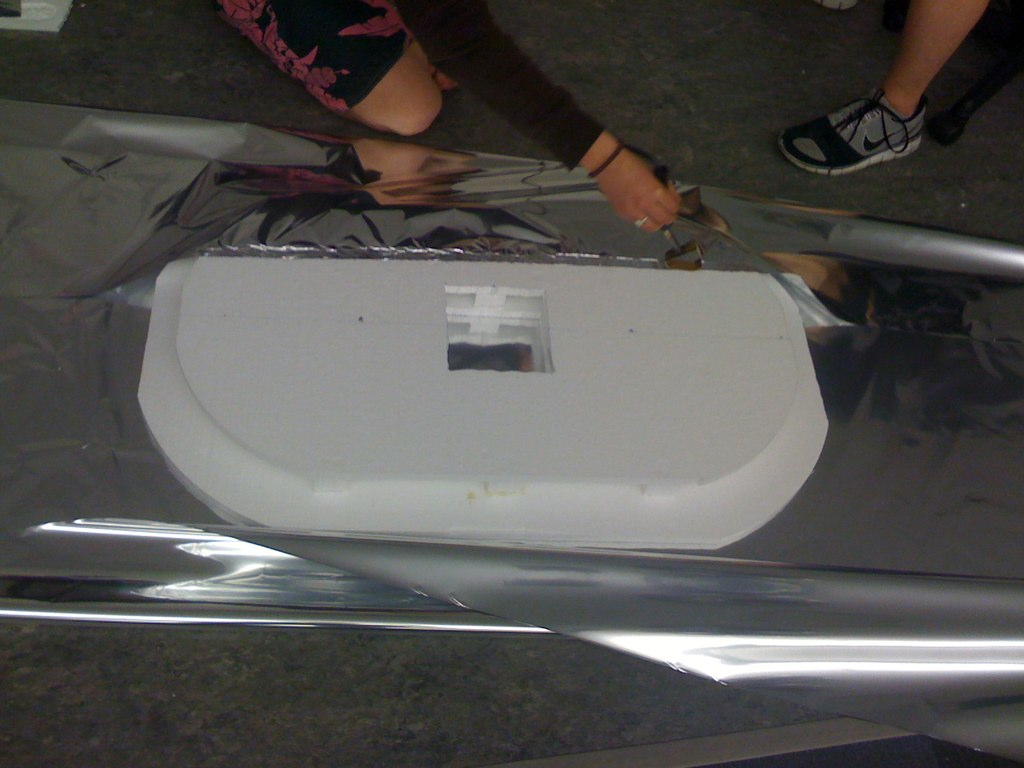
\includegraphics[width=85mm]{imageSources/rigidity1.png}
  \end{center}
  \caption{Rigidity of Hovercraft I} 
  \label{rigidity1}
\end{figure}

\begin{figure}[h]
  \begin{center}
    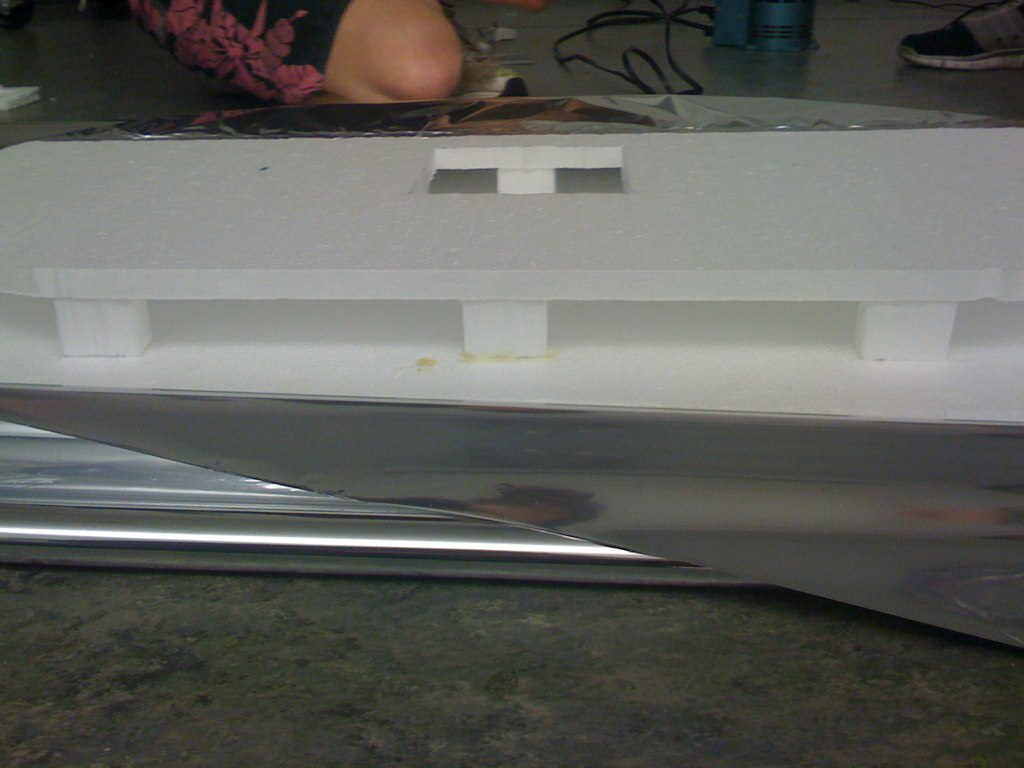
\includegraphics[width=85mm]{imageSources/rigidity2.png}
  \end{center}
  \caption{Rigidity of Hovercraft II} 
  \label{rigidity2}
\end{figure}

An inflatable skirt made of mylar surrounds the body. Mylar is a polyester film often used in flexible packaging for food, as an insulating material, and for solar reflection. Once inflated, the skirt serves two purposes. First, because it expands to over two inches, it provides additional surface area, reducing the overall pressure at any given point on the body. Second, the skirt acts as a flexible and damage resistant bumper, protecting the body from nearby objects during testing. We used two different mediums to connect the skirt to the styrofoam body. First we adhered the mylar to the styrofoam using hot glue, we then went around the perimeter with a hot iron to melt the mylar, the glue and the styrofoam together.

\begin{figure}[h]
  \begin{center}
    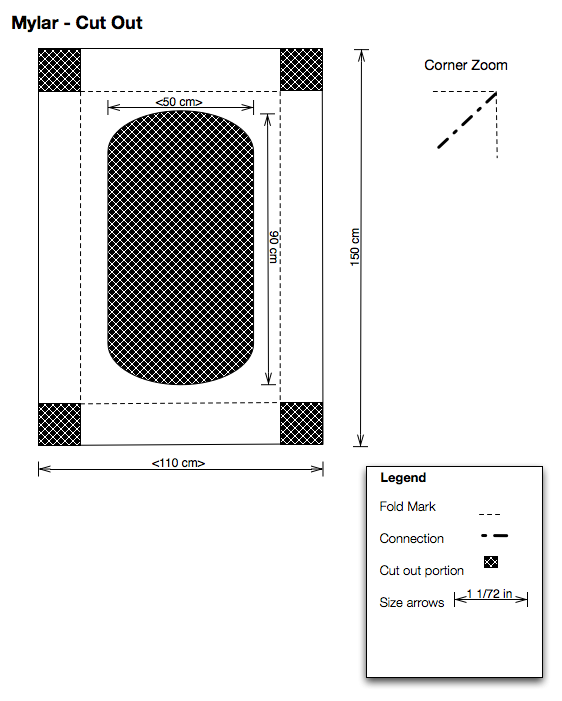
\includegraphics[width=85mm]{imageSources/mylarSchematic.png}
  \end{center}
  \caption{Schematic of the Mylar skirt} 
  \label{mylarSchematic}
\end{figure}

After the styrofoam chasis was built, we then procdeded to construct the skirt. The first attempt at constructing the mylar skirt was not successful. Lack of foresight resulted in a skirt that was too baggy in some areas, while exposing too many holes in others. The first time that we attached the mylar, when we were connecting the corners, we used clear packing tape, and simply folded the corners together. The second attempt was much more calculated and pragmatic. When connecting the corners of the second skirt, we methodically folded the edges in, then removed the square that was not attached (see Mylar-Cutout diagram). After this we made the connection using the hot iron to glue the seam together. The resulting skirt was much more evenly distributed and provided reasonably uniform inflation around the entire body. That said, the hovercraft still managed to move about when it was supposed to be idle. We addressed this issue by placing weights on the body to counteract the uneven escape of air on one side.

\subsubsection{Lift}
The decision to use a single, vertically mounted propeller to feed air into the plenum chamber was in direct response to the problem of rotational torque plaguing horizontally mounted propellers. In a horizontal design, the rotation of the blades applies an overall torque on the hovercraft causing it to spin. Dealing with this force is a burden. One approach is to install a second horizontal propeller which spins in the opposite direction. The opposite spin of the two motors cancels any directional torque felt by the craft. We chose to avoid this problem entirely by mounting a single motor vertically in the middle of the body. A container built over the propeller captures the incoming air and forces into the plenum chamber.

\begin{figure}[h]
  \begin{center}
    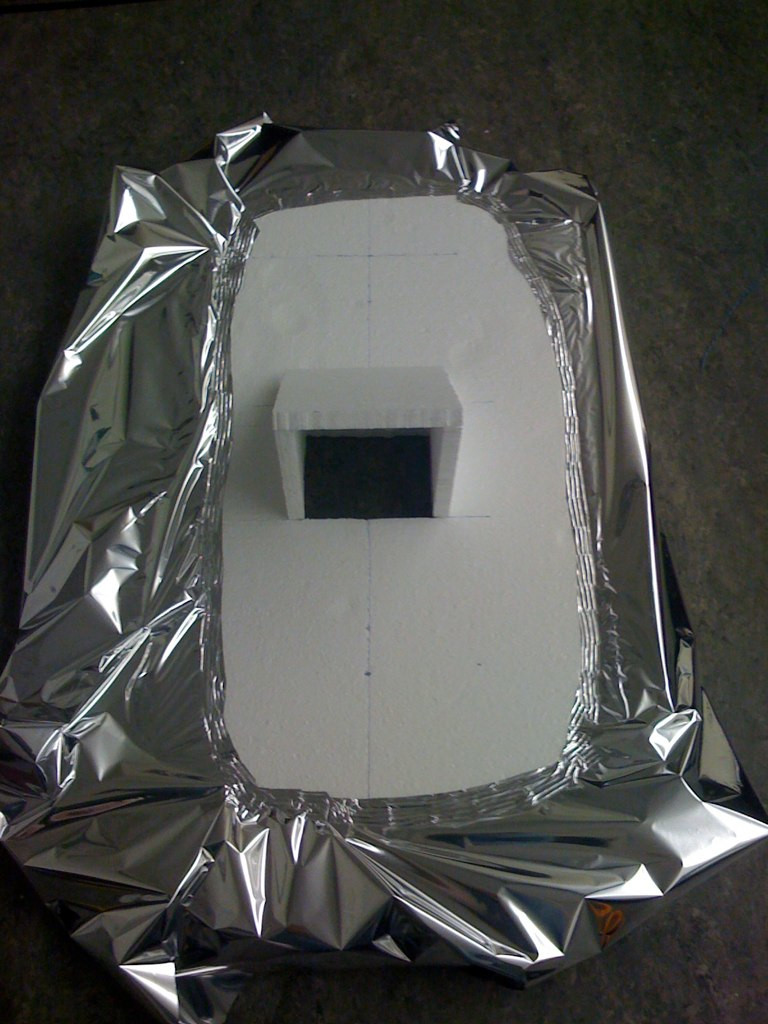
\includegraphics[width=85mm]{imageSources/lift1.png}
  \end{center}
  \caption{Hovercraft Lift I} 
  \label{lif1}
\end{figure}

\begin{figure}[h]
  \begin{center}
    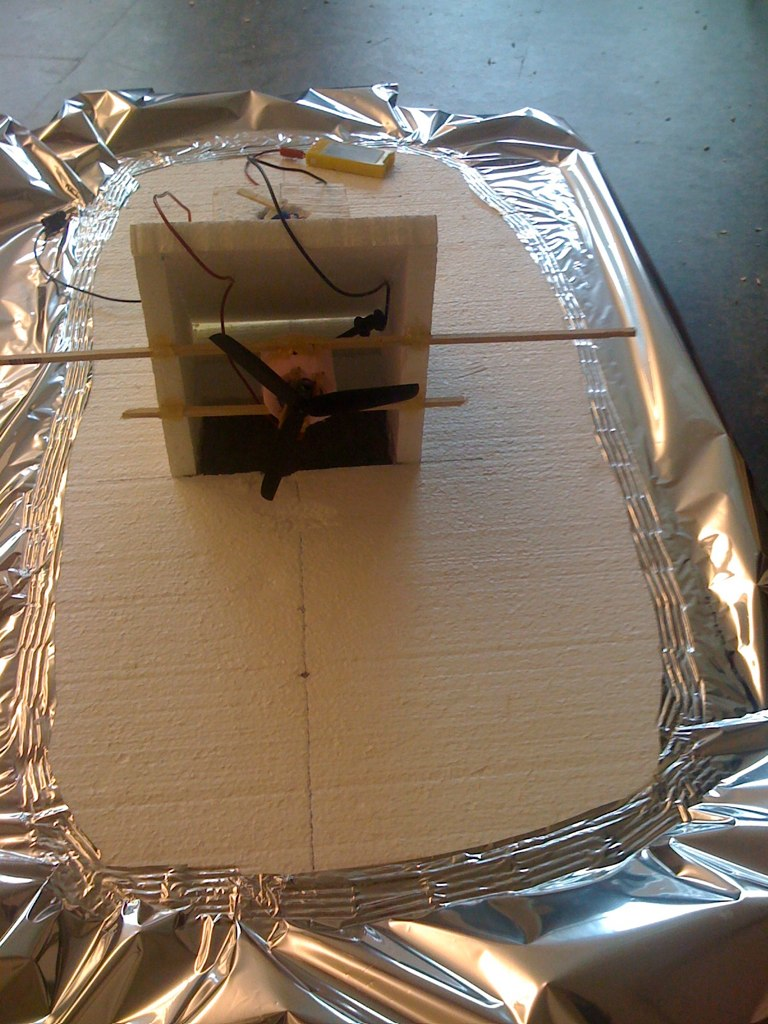
\includegraphics[width=85mm]{imageSources/lift2.png}
  \end{center}
  \caption{Hovercraft Lift II} 
  \label{lift2}
\end{figure}

To avoid ground effect, we applied full power to the lift propeller. Next, we methodically added weight to the body such that the hovercraft moved freely along the ground, but was not vastly overpowered by the fan. Keeping the vehicle as close as possible to the ground allows for the most control over the hovercraft's direction.

\subsubsection{Thrust and Control}

The following two figures show the first design we had chosen to provide the vehicle with thrust. The two differential motors were mounted at the rear, and were spaced fairly close together.

\begin{figure}[h]
  \begin{center}
    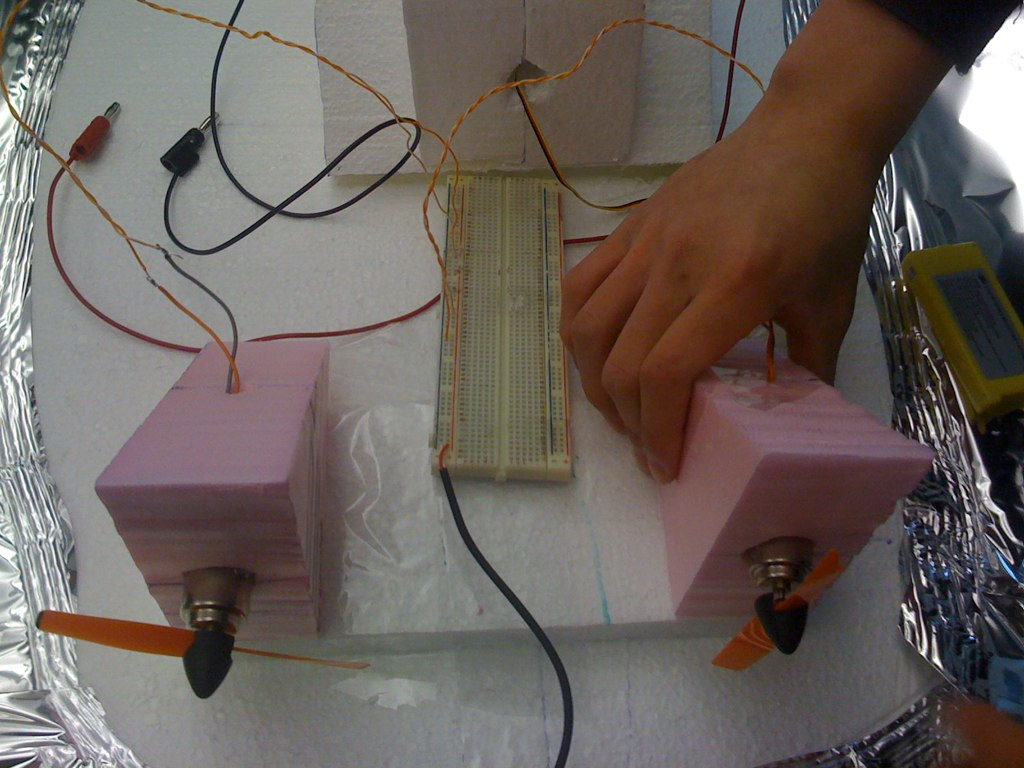
\includegraphics[width=85mm]{imageSources/thrustControl1.png}
  \end{center}
  \caption{Hovercraft Thrust and Control I} 
  \label{thrustControl1}
\end{figure}

\begin{figure}[h]
  \begin{center}
    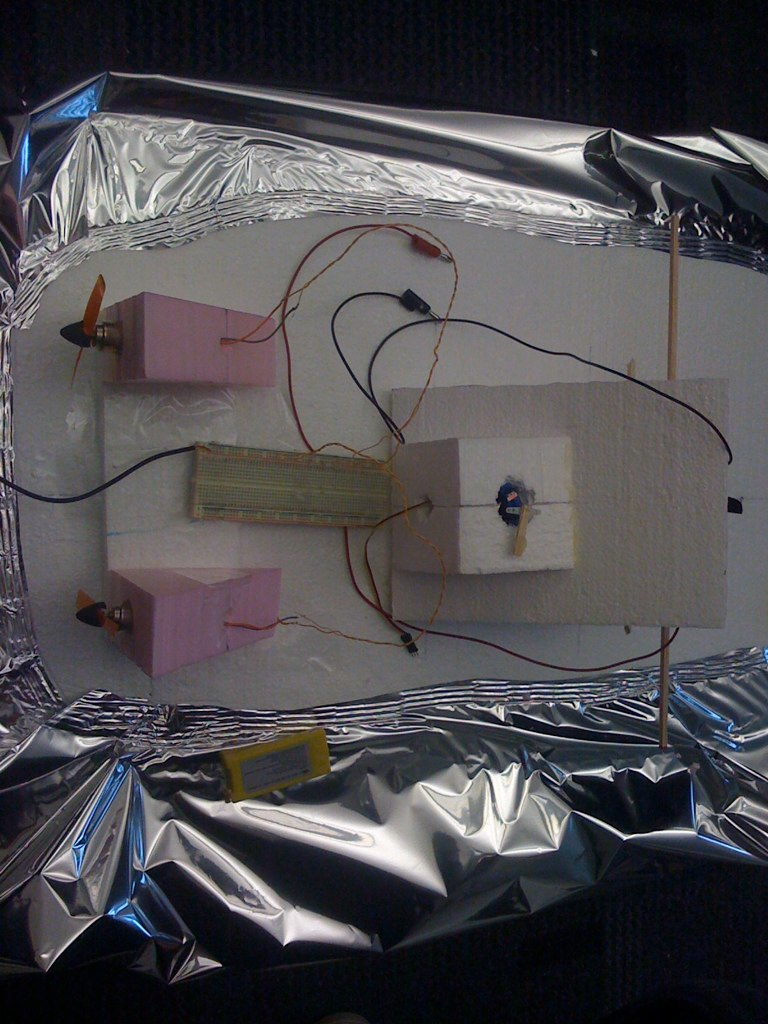
\includegraphics[width=85mm]{imageSources/thrustControl2.png}
  \end{center}
  \caption{Hovercraft Thrust and Control II} 
  \label{thrustControl2}
\end{figure}

We decided to change this design. By placing the motors as far apart as possible, maximum torque could be achieved. The analogy is as follows. Consider the act of opening a door. It is much easier to open a door if you push on the edge furthest from the hinges, because you can generate much more torque. The same goes for our hovercraft. Ideally the centre of rotation (the hinge) is in the centre of the hovercraft. By placing the motors as far away from this centre, we will create the most rotational torque and the craft will be easily controlled
